\documentclass[]{usiinfbachelorproject}


%Packages
\captionsetup{labelfont={bf}}
\usepackage[]{pdfpages}
\usepackage{tabularx}
\usepackage{algorithm}
\usepackage{algpseudocode}
\usepackage{imakeidx}
\usepackage{float}


%opening
\title{Rotation of multi-dimensional signals with spectrally accurate schemes}
\author{Dylan Reid Ramelli}



\versiondate{\today}

\begin{committee}
	\advisor[Universit\`a della Svizzera Italiana, Switzerland]{Prof}{Rolf}{Krause}
	\assistant[Universit\`a della Svizzera Italiana, Switzerland]{Dr}{Patrick}{Zulian}
	\assistant[Universit\`a della Svizzera Italiana, Switzerland]{Dr}{Diego}{Rossinelli}
\end{committee}

\abstract {
%	The idea to take on this project began on the assumption that rotating an image might be a considered a trivial task. It became clear that rotation is a multi faceted operation that involves different steps. First we must acquire the image and to do that we must be able to sense it. Just like a robot arm in an assembly line needs to know which parts of the car go where, we must be able to take a discrete sample from a continuous signal. Once the image is acquired we need tools that are as accurate as possible and immune to disturbances to be able to perform accurate rotations on the image. This project, which is based on a research paper on rotating images using a convolution based interpolation \cite{main_article} will try to explore a similar way to rotate an image while maintaining a high degree of accuracy and performance. To do this the Fourier Transform's property of shift and of convolution of a signal with a filter kernel will be taken advantage of. What will also be shown is how the filter kernel was created in the frequency domain and the problems that the choice of filter might pose to the result of the shift.
%	
}

\begin{document}	
	
	\maketitle
		
		
	\tableofcontents
	\newpage
	\section{Introduction, Motivation}\label{introduction}
	
	% Intro	
	\subsection{Light transport}
	In scientific image visualization there is a need to work with great magnitudes of data. We want to perform operations at this enormous scale because there might be some natural properties that might otherwise escape our ability to sense them.To be able to perform calculations on this much information we make use of high performing hardware with well defined structures.
	To visualize 3D models we calculate the amount of light that gets to one place from another. While light-rays traverse a model they suffer from attenuation, which is the property of any material that dictates how easily it can be penetrated by light. This property carries over to other forms of energy such as sound or particles.\\
	Since we deal with high amounts of data we must also use massive amounts of ray casting to light models correctly. 
	To carry out these calculations as efficiently as possible we can rotate the model to facilitate the arrangement of data through which the light has to pass through. This facilitates many tasks such as Multi-Modal imaging of computerized tomography (CT) scans and Positron Emission Tomography (PET) scans. While the former provides detailed structural images, the latter measures molecular activity and we can use image rotation to combine the two to capture other aspects of the structure. Another task that needs accurate data transformations is Data Augmentation for Convoluted Neural Networks (CNN).\\
	While 3D rotations make use of Euler angles to dictate the orientation of rotation, we can also express three dimensional rotations as a series of 2D rotations. This can be imagined as taking multiple slices of a model and rotating them by some degree. We can go even further by saying that a 2D image rotation can be expressed as three 1D signal translations in a cardinal direction\cite{main_article}. This notion is very powerful since it enables the creation of 1D schemes that can be used on almost any kind of hardware structure.\\
	The raw imaging data that is acquired provides us with multi-scale frequency components of the image. Our task is to manipulate the frequencies to obtain a higher fidelity rotation.
	
	
	\subsection{Manipulating frequency components of an image}
	Given that we can interpret 3D or 2D image rotation as a series of 1D translations we can define the scope of this project: we want to take a large scale signal and translate it by any real value, while maintaining a high level of accuracy and performance.\\
	To achieve this objective, we make use of filter convolution and frequency component analysis in the Fourier domain.
	Our code will be efficient and minimalist in order to ensure high performance on any kind of hardware. 
	
%	\subsection{2D rotations as 1D translations}
%	Starting from a reference paper \cite{main_article} we found that 2D rotations can be simply expressed as 1D translations by modifying the traditional rotation matrix.

	
%	What is the contribution in the project: How to create a filter, show implementation and maybe study the numerical performance
%	Accurate rotation requires the use of some fundamental signal processing concepts: Fourier domain and convolution of a signal with a filter. Filters are necessary in this work for their simplicity and ease of computational complexity. It will be shown how to create a filter to use as kernel for convolution with the original signal to rotate by fractional amounts. Something that is quite difficult to do accurately with traditional methods of interpolation for example. 
	
	%Motivations
	
%	\subsection{Applications}
%	This work could become very useful in many applications that rely on accurate signal rotations such as Data Augmentation for example. In this case we want to increase the coverage of a certain dataset. In Convoluted Neural Networks we can augment the dataset by rotating the input images by some random rotation and then feeding them to the model to improve it without having to collect more data externally.
%	Another application of this technique can be seen in Data Visualization for multi-modal imaging. Images are taken at different times or in different ways, such as in a PET-CT scan and rotation can enable us to re-align the elements present in these images. In this case we can either acquire images at different times and then combine them together so that we can manipulate the images by rotation for example to align them correctly. Go into more detail.. ask Diego.
	
	
%	\subsection{Contributions}
%	The goal of this project is to process high quality multi-dimensional signals, by rotating them by any angle using techniques such as the Fourier Transform and filter convolution.


	\begin{figure}[h]
	\centering
	\includegraphics[width=0.9\columnwidth]{images/homeostasis-log-v2.jpg}
	\caption{Large-scale in-silico investigation of homeostasis in the subarachnoid space of the human optic nerve [Rossinelli et al. 2023, in-preparation]. Homeostasis is directly related with the interaction between the cerebrospinal fluid flow (not shown here) and the meningeal surface. Blue denotes poor levels of homeostasis , whereas red denotes sufficient material exchange between fluid and structure.}
	\cite{main_article}
	\end{figure}
	
	\iffalse
	
	\subsection{Interpolation}
	Sampled version of our translated signal is:
	\begin{equation}
		(T_\Delta s)[k] = \sum_{l \in Z}^{} c(l)\varphi(k - \Delta - l)
	\end{equation}
	Where $\varphi$ is our generating function.
	\subsubsection{Linear Interpolation}
	With linear interpolation we want to estimate the coordinates of a point from a given number of samples. 
	
	Linear interpolation model of function sin(x) with $N = 2$:
	\begin{equation}
		\beta^1(x) = 
		\begin{cases}
			1 - |x|, & |x| < 1    \\
			0,       & otherwise, 
		\end{cases}
	\end{equation}
	\begin{center}
		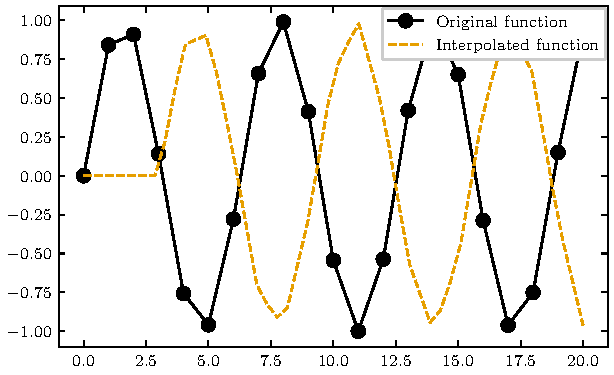
\includegraphics{"images/linear_interpolation_example.pdf"}
	\end{center}
	
	Cubic spline interpolation model of function sin(x) with $N=4$:
	\begin{equation}
		\beta^3(x) = 
		\begin{cases}
			2/3 - |x|^2 + |x|^3/2, & 0 \leq|x| < 1  \\
			(2-|x|)^3/6,           & 1 \leq |x| < 2 \\
			0,                     & 2 \leq |x|     
		\end{cases}
	\end{equation} \cite{main_article}
	
	\begin{center}
		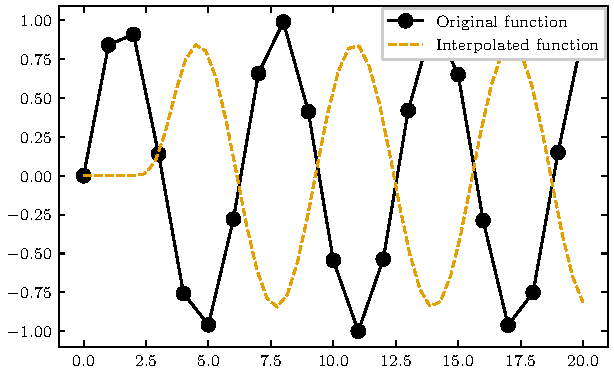
\includegraphics{"images/cubic_interpolation_example.pdf"}
	\end{center}
	
	Standard 2-D interpolation formula for computing the value of the image at location $(x,y)$
	\begin{equation}
		s(x,y) = \sum_{k = k_0}^{k_0+L-1}\sum_{l=l_0}^{l_0+L-1} c(k,l)\varphi(x-k)\varphi(y-l)
	\end{equation}
	
	\fi
	

	\section{Methodology}	
		As stated in the introduction we will take advantage of the fact that a 2D rotation can be expressed as a 1D translation which we reference from this article \cite{main_article}. 
		In the case of the article the authors propose the use of different convolution-based interpolation schemes such as polynomial splines of degree $n$, cubic spline, etc. to translate a 1D signal. These operations are inherently global, which is not particularly effective since translation is a fundamentally local operation.
		In our case however we will perform local direct convolutions on the original signal with a filter, whose frequency components we manipulate in the frequency domain.
%		In \cite{main_article} these translations are performed by downsampling the image before performing B-spline interpolations to shift the signal. The interpolation is done to flatten out the spurious oscillations that are due to high order 
		 To create our own convolution filter in the frequency domain we will start with the Discrete Time Fourier Transform of a cosine function in an interval $[-M,M]$ . Defining the function in the Fourier space allows us to fine tune the filter to have a better control over the smoothing effect that will occur when we shift by fractional amounts. The filter is small compared to the original signal. Finally we will perform direct convolution of the signal with the computed filter.
		 
		 \subsection{2D rotation as 1D translation}
		 As stated above, in the article that this project takes inspiration from, it is shown that the traditional rotation matrix
	\begin{equation*}
		R(\theta) = 
		\begin{pmatrix}
			cos\theta & -sin\theta\\
			sin\theta & cos\theta
		\end{pmatrix}
	\end{equation*}
	can be factorized as three matrices each of which represents a shearing of the image in a cardinal direction.
	\begin{equation}\label{3_translations}
		R(\theta) = 
		\begin{pmatrix}
			cos\theta & -sin\theta\\
			sin\theta & cos\theta
		\end{pmatrix}
		=
		\begin{pmatrix}
			1 & -tan\theta/2\\
			0 & 1
		\end{pmatrix}
		\cdot
		\begin{pmatrix}
			1 & 0\\
			sin\theta & 1
		\end{pmatrix}
		\cdot
		\begin{pmatrix}
			1 & -tan\theta/2\\
			0 & 1
		\end{pmatrix}
	\end{equation} 
	
	The first matrix shears the image in the $x$ direction by $\Delta_x = -y\cdot tan(\theta/2)$, the second matrix shears the image in the $y$ direction by $\Delta_y = x \cdot sin(\theta)$ and the last matrix shears the image again in the $x$ direction by $\Delta_x$.
%	In our case we can represent the image as a one dimensional array ordered row-wise. 
	
	\begin{figure}[H]
		\centering
		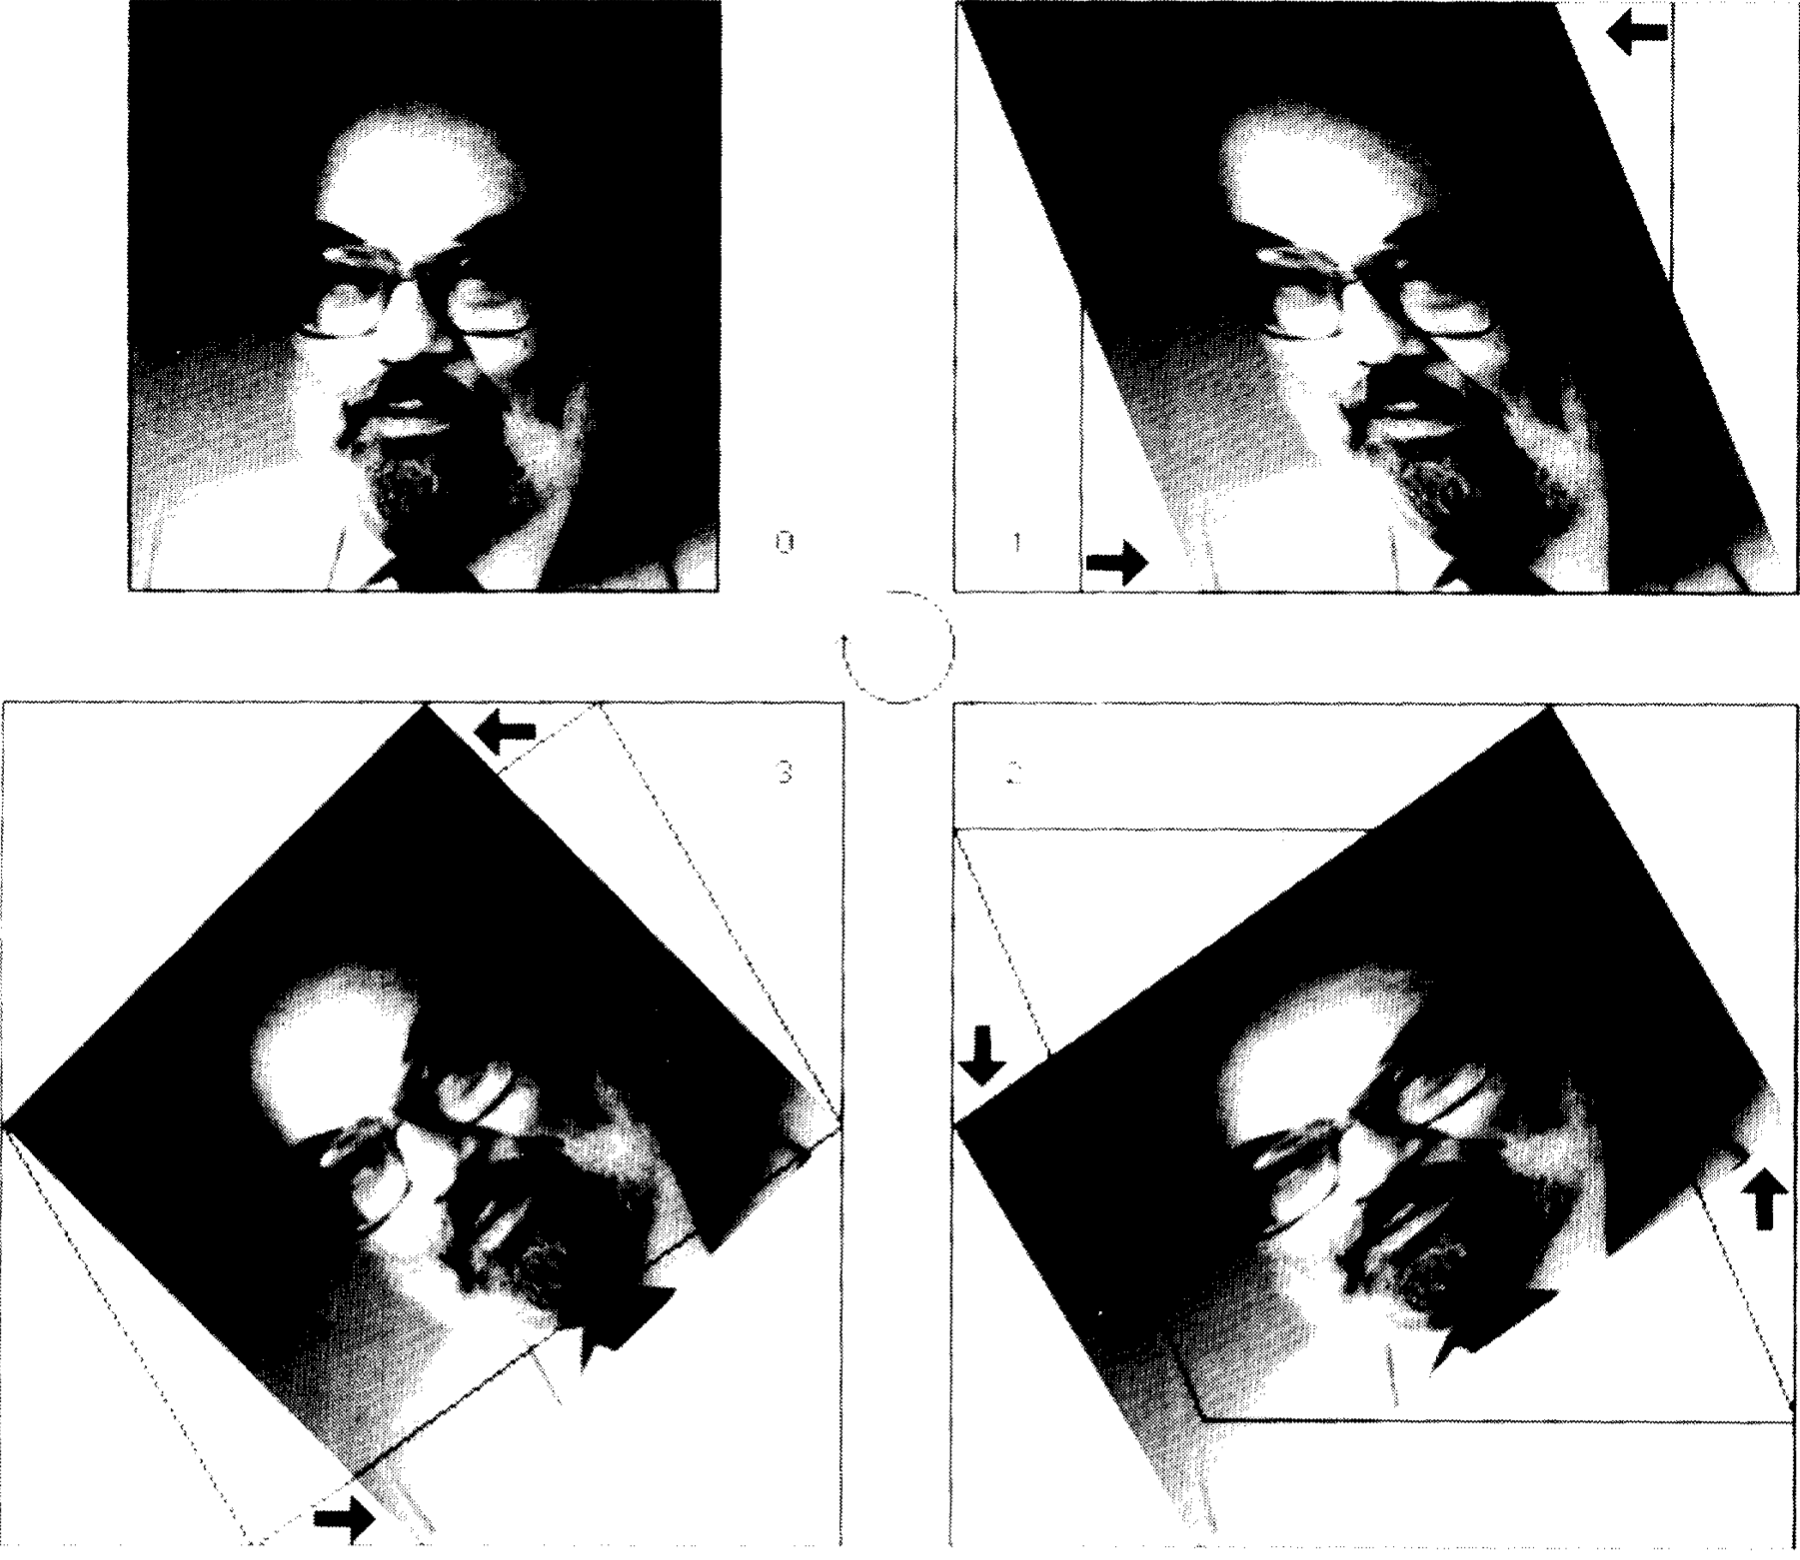
\includegraphics[width=0.5\columnwidth]{images/unser_rotation.png}
		\caption{Rotation of an image done with 3 1D translations.}
		\cite{main_article}
	\end{figure}
	
		
	\subsection{Fourier Transform}
	In signal processing working in the frequency domain has a great advantage since any function that is expressed in this way can be reconstructed completely via an inverse process, with no loss of information.\cite{image_book}
	For a function $g(x)$ to be represented in the frequency domain we must then use of the Discrete Fourier Transform (DFT), which is defined as follows:
	\begin{equation}
		G_m = \displaystyle\sum_{k=0}^{N-1}g_ke^{-i \frac{2\pi}{N}km}
	\end{equation}
	
	In this project the above equation will not be used since the filter that is going to be defined in one of the next chapters, will be created directly in the Fourier domain. Nevertheless it is useful to show the definition since it is the Inverse Discrete Fourier Transform that will be used to reconstruct the filter in the time domain:
	\begin{equation}
		g_n = \frac{1}{N}\displaystyle\sum_{k=0}^{N-1}G_ke^{i \frac{2\pi}{N}kn}
	\end{equation}
	
	
	\subsection{Derivation of the shift interpolant}
	Here we derive the shift filter for a discrete signal starting from the normal Fourier Transform with $f$ being our 1D input array, $N$ the number of samples and $m$ the frequency:
	\begin{equation*}
		F_m = \displaystyle\sum_{k=0}^{N-1}f[k]e^{-i \frac{2\pi}{N} km}
	\end{equation*}
	
	Now instead of $f[k]$, we want $f[k - \delta]$ where $\delta$ is the amount we want to shift.
	So the above equation can be rewritten as:
	\begin{equation*}
		Z_m = \displaystyle\sum_{k=0}^{N-1}f[k - \delta]e^{-i \frac{2\pi}{N} km}
	\end{equation*}
	
	\begin{equation*}
		Z_m = \displaystyle\sum_{r = 0 - \delta}^{N-1-\delta}f[r]e^{-i \frac{2\pi}{N} km}, r = k - \delta 
	\end{equation*}
	
	Since $r = k - \delta$ then $ k = r + \delta$, and as such:
	
	\begin{equation*}
		Z_m = \displaystyle\sum_{r= -\delta}^{N-1 - \delta}f[r]e^{-i \frac{2\pi}{N} (r + \delta)m}
	\end{equation*}
	
	We can then separate the exponential:
	
	\begin{equation*}
		Z_m = \displaystyle\sum_{r= -\delta}^{N-1 - \delta}f[r]e^{-i \frac{2\pi}{N} rm}e^{-i \frac{2\pi}{N}  \delta m}
	\end{equation*}
	
	And factor it out of the sum:
	
	\begin{equation*}
		Z_m = e^{-i \frac{2\pi}{N}  \delta m} \displaystyle\sum_{r= -\delta}^{N-1 - \delta}f[r]e^{-i \frac{2\pi}{N} rm}
	\end{equation*}
	
	\begin{equation*}
		Z_m = e^{-i \frac{2\pi}{N}  \delta m} \displaystyle\sum_{k=0}^{N-1}f[k]e^{-i \frac{2\pi}{N} km}
	\end{equation*}
	
	\begin{equation}
		Z_m = e^{-i \frac{2\pi}{N}  \delta m} F_m = H_m \cdot F_m \label{shift_equation}
	\end{equation}
	
	\subsection{Interpretation of frequencies for fractional shifts}
	The final equation from the previous section \ref{shift_equation} works well for any integer shifts that we want to perform on our signal but for any fractional amount we encounter some problems with the use of the correct frequency indexes.

	
%	And we can see that from $N/2$ we start getting negative values for the  magnitutde of each frequency. These negative values correspond the the complex conjugate of each frequency.
	
	As stated in equation \ref{shift_equation} we multiply each sample by its corresponding phase, which is based on the frequency number $m$.
	We need to take into consideration the negative frequencies for fractional shifts  and as such we can define a function called wavenum that returns the correct frequency index to use:
	\begin{equation*}
		wave\_n(m) = (m + \lfloor N/2 \rfloor ) \bmod N - \lfloor N/2 \rfloor
	\end{equation*}

	\begin{figure}[H]
		\centering
		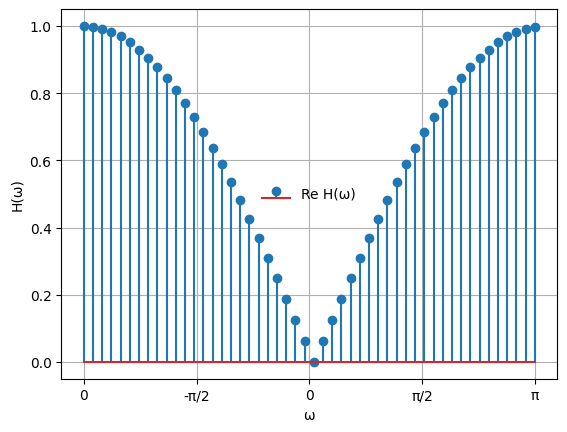
\includegraphics[width=0.5\columnwidth]{images/good_shift_filter.png}
		\caption{Shift filter of size $n=50$, with a fractional shift of $\delta=0.5$}
	\end{figure}
	Modify original equation to use wavenum.
	\begin{equation*}
		H(\omega) = e^{-i \frac{2\pi}{N}  \delta wave\_n(m)}
	\end{equation*}
	\begin{equation}\label{phase_shift_equation}
		Z_m = e^{-i \frac{2\pi}{N}  \delta m} F_m 
	\end{equation}	
	
%			DFT^{-1} (\{H(\omega_{i}) F(\omega_{i})\}_i)
	
	
	\subsection{Smoothing Filter (Low-Pass)}
	The smoothing filter is what we will use to alleviate the oscillations that occur with fractional shifts.
	To start off we define the filter in the Frequency domain with the use of the Continuous Fourier transform (CFT)on a cosine function.
	\begin{equation}
		F(\omega) = \int_{-M}^{M} \cos(\frac{\pi}{M}t)\mathrm{e}^{-\mathrm{i}\omega t}\mathrm{d}t
	\end{equation}
	This equation allows us to define our CFT in an interval $M$, that we choose based on the fractional amount we want to shift. The interval M is useful to us to fine tune the filter and choose how big of a smoothing effect we want.
	\begin{equation}\label{filter_formula}
		F(\omega) = \frac{2M^2\omega \sin(M\omega)}{M^2\omega^2-\pi^2}
	\end{equation}
	
	Using this function we can build the following filters for each M:
	
	% Filters.
	\begin{figure}[H]
		\centering
		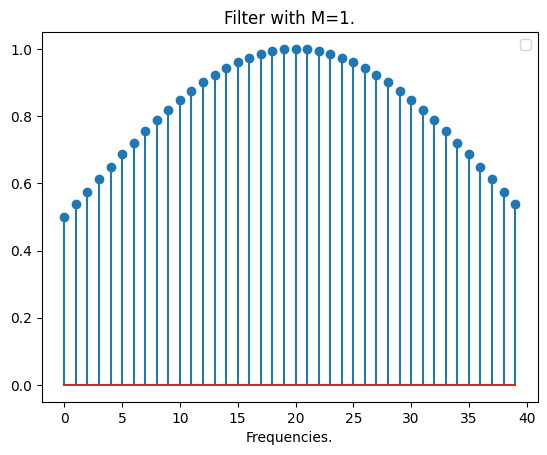
\includegraphics[width=0.4\columnwidth]{images/filter_m_1.png} \hfill		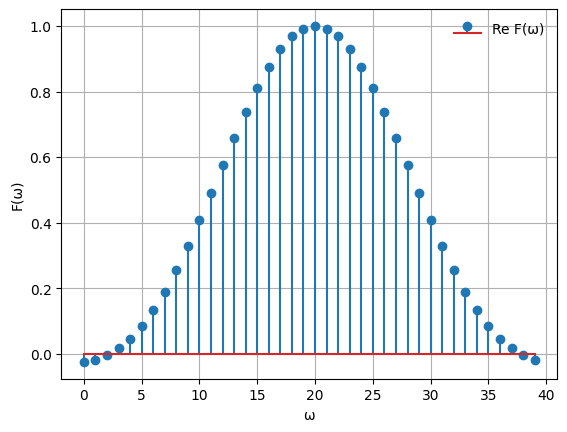
\includegraphics[width=0.4\columnwidth]{images/filter_m_1_5.png} \\
		\parbox{0.4\columnwidth}{\centering Filter with M = 1.} \hfill
		\parbox{0.4\columnwidth}{\centering Filter with M = 1.5.}
		\centering
		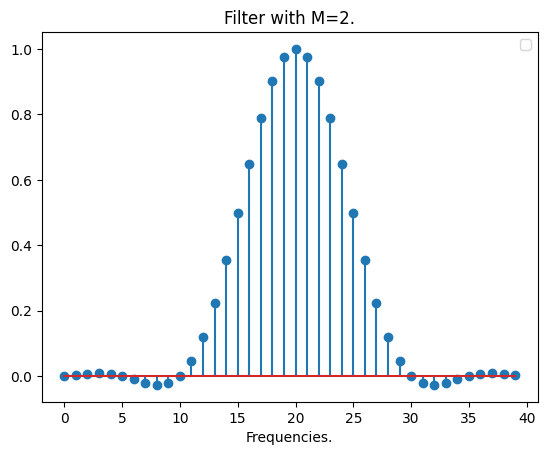
\includegraphics[width=0.4\columnwidth]{images/filter_m_2.png} \hfill		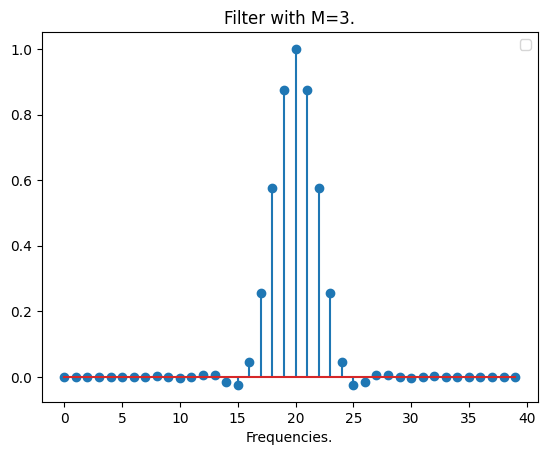
\includegraphics[width=0.4\columnwidth]{images/filter_m_3.png} \\
		\parbox{0.4\columnwidth}{\centering Filter with M = 2.} \hfill
		\parbox{0.4\columnwidth}{\centering Filter with M = 3.}
		\caption{Compact schemes of different M for local computation (DTFT).}
		\label{filters}
	\end{figure}
	%
	
%	In figure \ref{filters} we can see the general shape of the function for each M and the number of samples it will use for convolution. 
%	It does not however give us a good idea on how it is going to modify the signal. In the next figure we can see the same filters but in the time domain.
	% Filters. % impulse reposne
	
	For better accuracy we generally choose our interval M to be small when we have a small fractional shift and big when we have a shift that gets closer to $0.5$. We can write a simple expression that defines M in respect to the fractional shift $x$ to be:
	
	
	% Tenere?
	\begin{equation*}
		M = 
		\begin{cases}
			1.5 & if 0.1 < x < 0.3\\
			2 & if 0.3 < x < 0.5
		\end{cases}
	\end{equation*}
	
	With some experimenting we found that the filter with $M=3/2$ is a good compromise between smoothing the values and keeping them as accurate as possible.
	
	\subsection{Creating a Filter in the Frequency domain}
	In this section we propose an example of the smoothing filter.
	We will create one of size $40$ with $M=2$. We then follow equation \ref{filter_formula}, while also paying attention to evaluating the limit when $\omega=\frac{\pi}{M}$ or $\omega=-\frac{\pi}{M}$. This gives us:
	\begin{figure}[h]
		\centering
		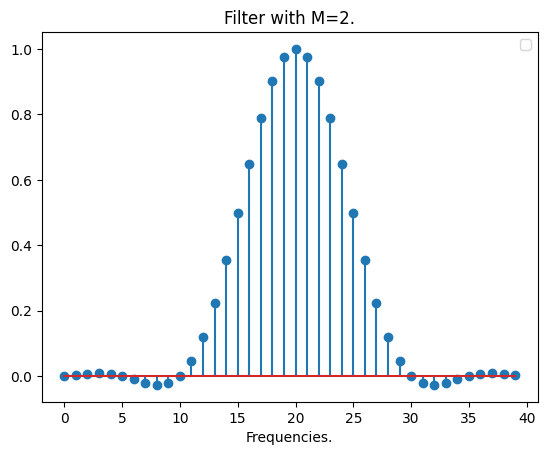
\includegraphics[width=0.4\columnwidth]{images/filter_m_2.png}
		\caption{Filter with $M=2$}
		\label{original_filter}
	\end{figure}
	
	Now let us say that the fractional amount to shift is $0.25$. We then multiply our smoothing filter $F(\omega)$ by our shift filter $H(\omega)$.
	\begin{figure}[h]
		\centering
		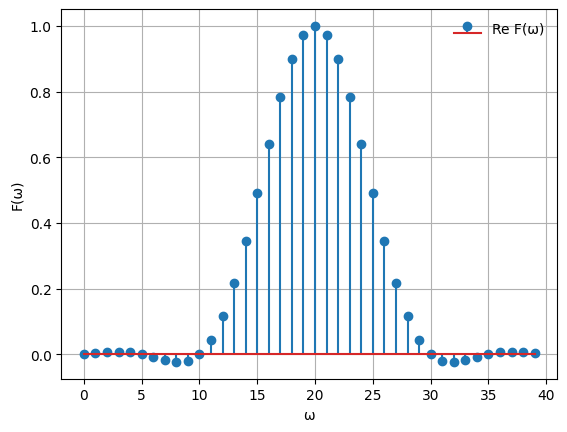
\includegraphics[width=0.4\columnwidth]{images/filter_m_2_25_shift.png}
		\caption{Filter with $M=2$ after shift of $0.25$}
		\label{shifted_filter}
	\end{figure}
	
	
	Finally we do an Inverse Fourier Transform to acquire our filter in the time domain.
%	Afterwards we implemented a simple version of the inverse Fourier transform, which give us our signal in the time domain. Before returning the result however we need to perform the equivalent of numpy's fftshift function to have the filter values centered. This whole operation can be done in serial and with no real optimization of the code since the kernel size will always be much smaller than the input signal and as such will no be computationally expensive.
	\begin{figure}[h]
		\centering
		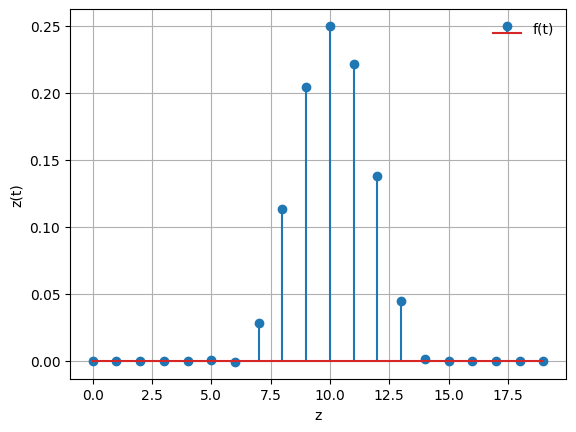
\includegraphics[width=0.4\columnwidth]{images/ifft_filter_m_2_25_shift.png}
		\caption{Filter with $M=2$ in time domain.}
		\label{final_filter}
	\end{figure}
	
	
	
%	Here is some pseudo-code that explain what is being done to our original filter:
%	\begin{algorithm}
%		\caption{Filter shift}\label{alg:cap}
%		Write convolution algorithm defined with compiler explorer
%	\end{algorithm}
%	
	
	\iffalse

	
	\begin{figure}[h]
		\centering
		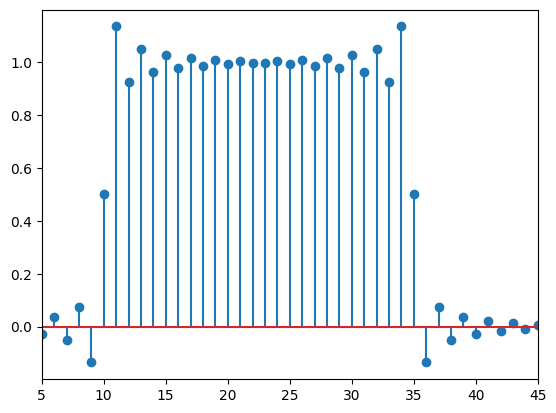
\includegraphics[width=0.5\columnwidth]{images/box_shifted_delta10_1_n50.png}
		\caption{Shifted function by $\delta=10.5$}
	\end{figure}
	
	\subsection{Lanczos Filter and FIR}
	To alleviate the problems that arise when shifting a signal by a fractional amount we can use a filter $L$ that is convoluted with the shifted signal.
	
	\begin{align*}
		L_m &= \frac{\sin(a)}{a},\\
		a &= \frac{2\pi wave\_n(m)}{N}
	\end{align*}
	
	Apply lanczos filter to fractional shift to smooth the result.
	
	\begin{equation*}
		Z_m = L_m \cdot H_m \cdot G_m
	\end{equation*}
	
	\begin{figure}[h]
		\centering
		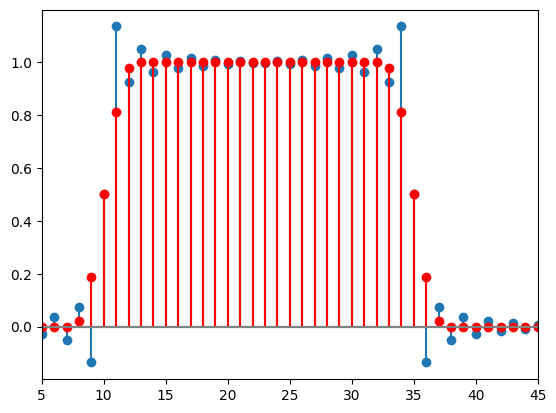
\includegraphics[width=0.5\columnwidth]{images/box_shifted_lanczos_delta10_1_n50.png}
		\caption{Shifted function by $\delta=10.5$ with lanczos filter applied (red), no filter(blue).}
	\end{figure}
	
	\fi
	
	
	\section{Implementation and Project Design}
	
%		\begin{itemize}
%			\item creazione filtro e spiegare perche IFT invece di ifft
%			\item perche direct convolution invece di fft
%			\item code generation at compile time with python script
%			\item piccola spiegazione su SIMD e metodo di convoluzione per facilitare la vettorizzazione dell'assembly code
%		\end{itemize}
	
		We chose a bottom-up approach for this project since we saw that the implementation steps were well suited for it. 
		We started with the fundamentals of signal processing by exploring the Fourier Transform and its properties to build our shift filter. We used Jupyter Notebook extensively to test our method and quickly plot the results, while also documenting everything so that it would be easier to complete this report. Since we used the bottom-up approach we were able to re-use parts of the code to test some other aspect of the shift. We started with simple shifts of a 1D signal by an integer values then we tried to shift the same signal by a fractional amount. This is where some problems arose with the usage of the correct frequency index but in code we easily implemented it with a basic method. The source code of this project is available at: \url{https://github.com/DylanReidRamelli/Bachelor-Project-2023}.
		The tools that were used: MakeFile, CMake, Jupyter Notebook and some built-in libraries of C and Python like numpy and matplotlib.
		
	\subsection{Libraries}
		Numpy and Matplotlib were a huge help in visualizing the results of the Fourier Transform and of the shifts. These libraries were also useful for when we started writing code in C. Where we would output the binary result to a file and then read it and plot the result in python. There are a few plotting libraries for C like the gnuplot library but we felt that this was just the faster/easier solution.
		The whole project started out as a CMake and this was chosen mainly because I was already familiar with this tool and was able to quickly setup an environment that would build the executable. However towards the end we decided to just use a plain Makefile to keep everything nice and simple. The added advantage of the makefile was to be able to easily run a python script at compile time to create other files needed by the main target. 
		 
		
		\subsection{Efficient implementation of direct convolution on x86 microarchitectures}
		Once the filter creation is done we must retrieve the signal in the time domain and to do this we implemented the "slow" version of the Inverse Fourier Transform since the size of the operation will always be much smaller than the original data.
		To keep our one dimensional direct convolution as simple and as efficient as possible we analysed it using a Web tool called "Compiler Explorer"\cite{godbolt}. This tool allows us to see which assembly code is being used to perform the convolution operation and choose which implementation should run faster on certain compilers and CPU's.
		
		\begin{figure}[h]
			\centering
			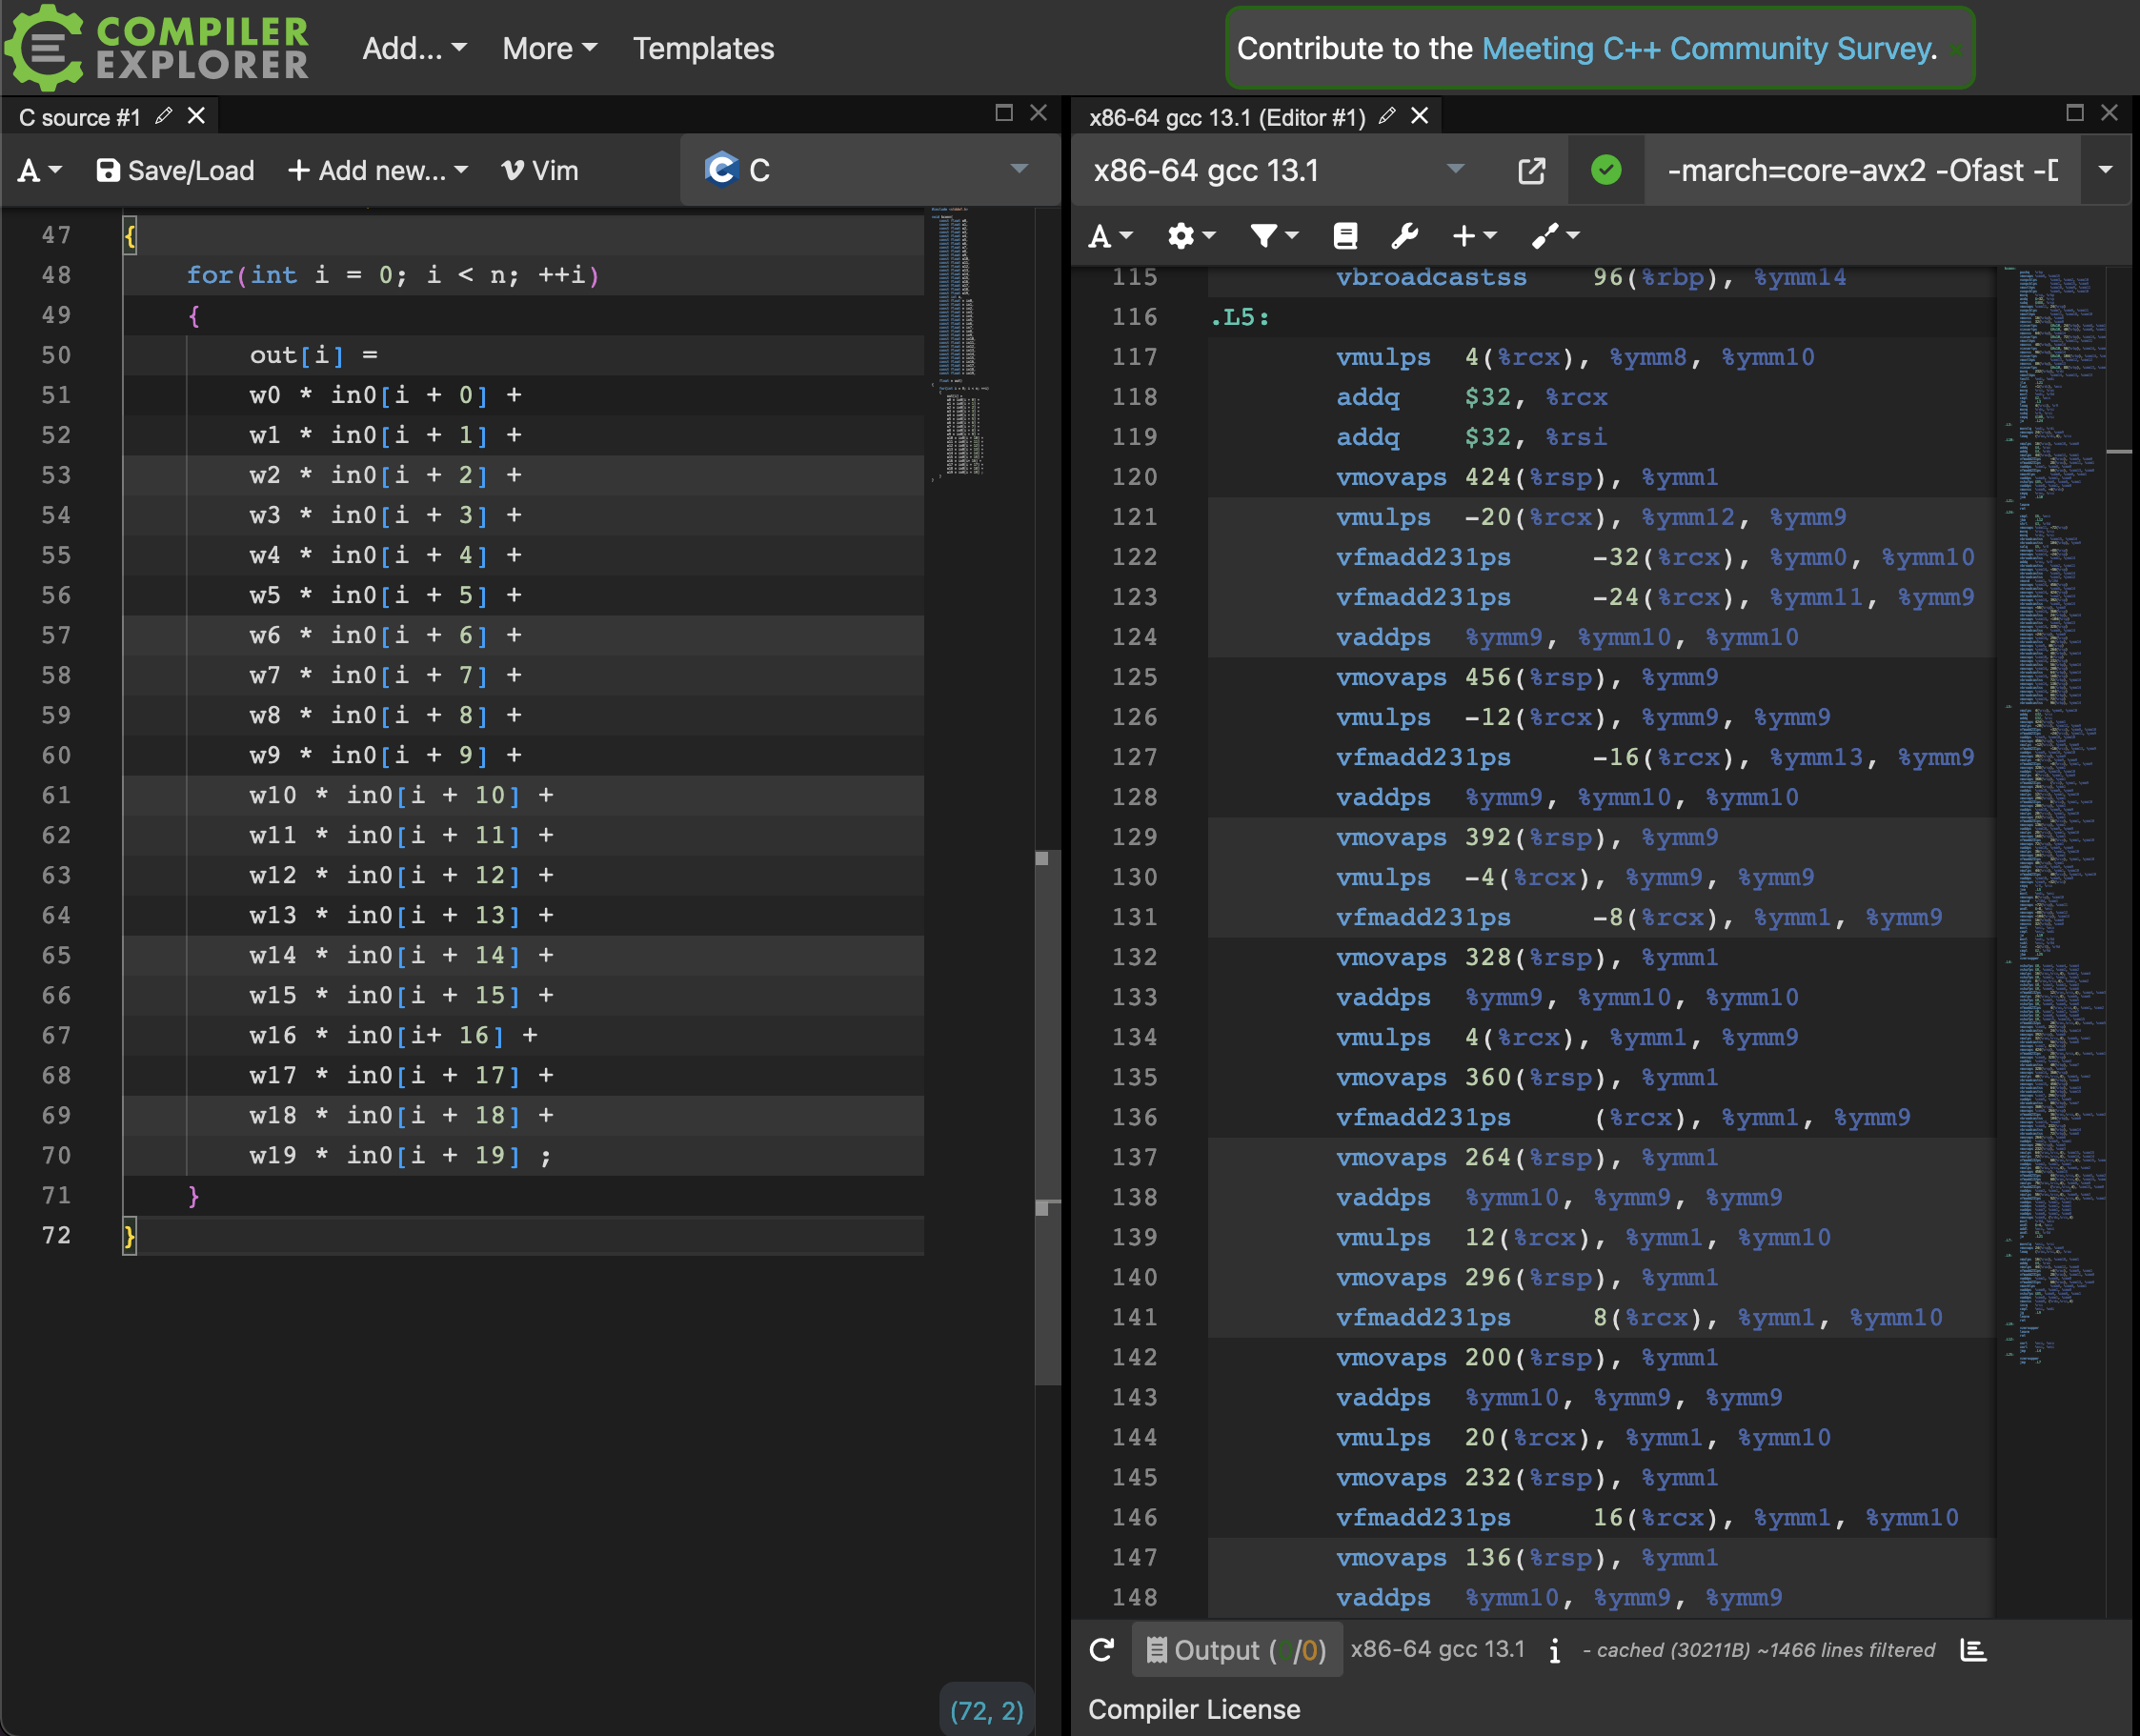
\includegraphics[width=1\columnwidth]{images/godbolt.png}
			\caption{Convolution function as seen in Compiler Explorer}
			\label{godbolt}
		\end{figure}
				
		
		
		The code that we came up with is easily written by a python script that is called at compile time by the make file, the only parameter we define is the size $M$ that we want to use and the script will generate a header and source file in C that will be used for the convolution.
		
		
		
		\subsection{Integer Shift} 
		Now that the fractional part of the shift has been taken care of we need to shift the signal by the integer value.
		First of all it should be clarified that if the shift does not have a fractional part then we skip the convolution with the filter entirely.
		To shift a signal by an integer amount we used the C function \textsl{memcpy} to copy the values of the original array to a resulting array but at a different position, which is defined by the integer shift. We chose \textsl{memcpy} instead of just moving the values inside the same array with \textsl{memmove} since \textsl{memcpy} is designed to be the fastest library routine to copy data from memory to memory.
		
		\newpage
		\section{Results}
		\subsection{Results with 1D signals.}
		One dimensional signals are the starting point of our tests and as such we chose a pretty aggressive signal to test out. In this example we are using a starting signal of binary value of length $n=100$ samples and it is defined as:
		\begin{equation*}
			f(x) = 
			\begin{cases}
				1	& \quad \text{if } x \leq \frac{n}{2}\\
				0	& \quad \text{otherwise}
			\end{cases}
		\end{equation*}
		\begin{figure}[h]
			\centering
			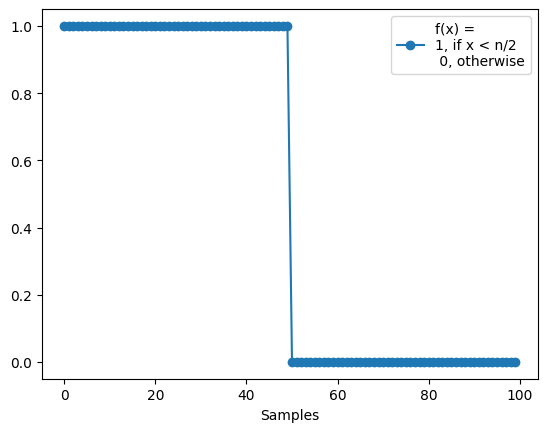
\includegraphics[width=0.4\columnwidth]{images/original_signal.png}
			\caption{Original signal of size $n=100$ samples.}
			\label{original_signal}
		\end{figure}
		
		By taking this signal and shifting it by $20.25$ we get a different result depending on the M chosen when creating the filter.
		\begin{figure}[H]
			\centering
			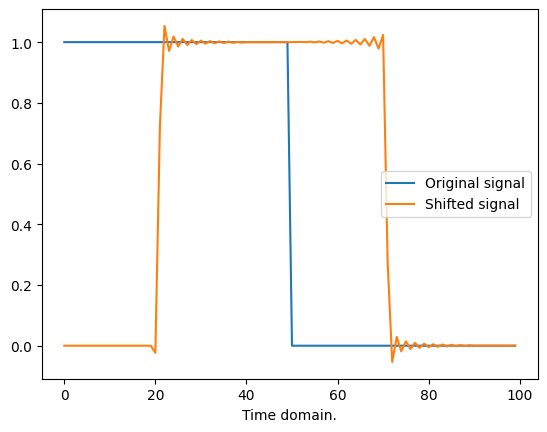
\includegraphics[width=0.3\columnwidth]{images/Results/M_1.png}\hspace*{0.2\columnwidth}
			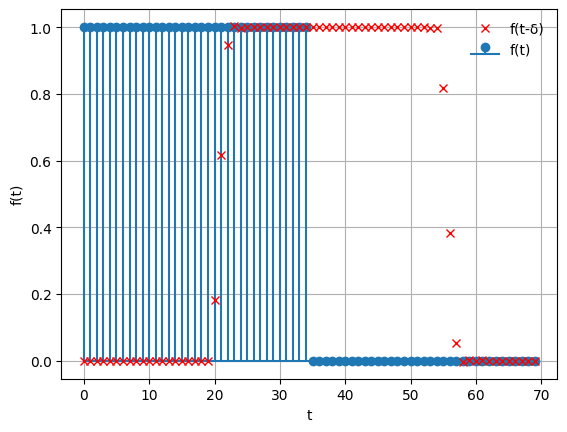
\includegraphics[width=0.3\columnwidth]{images/Results/M_3_2.png}\\
			\parbox{0.3\columnwidth}{\centering Filter with M = 1.}\hspace*{0.2\columnwidth}
			\parbox{0.3\columnwidth}{\centering Filter with M = 3/2}\\
			\centering
			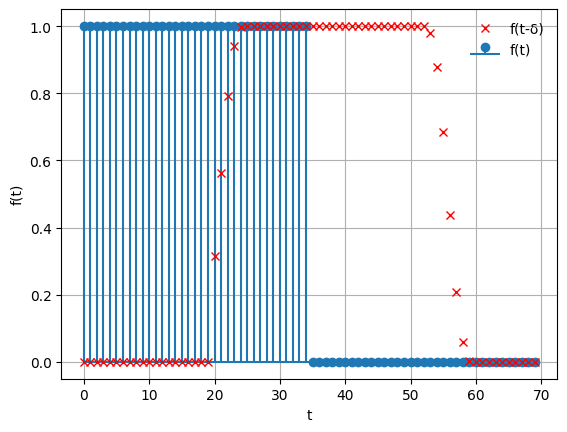
\includegraphics[width=0.3\columnwidth]{images/Results/M_2.png}\hspace*{0.2\columnwidth}
			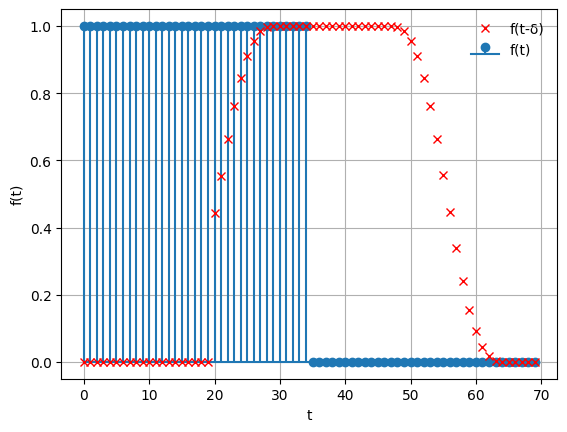
\includegraphics[width=0.3\columnwidth]{images/Results/M_3.png} \\
			\parbox{0.3\columnwidth}{\centering Filter with M = 2.}\hspace*{0.2\columnwidth}
			\parbox{0.3\columnwidth}{\centering Filter with M = 3.}
			\caption{Shift by 20.25}
			\label{results_1}
		\end{figure}
		
		At first glance we can see that with $M=1$ we have too many oscillations present in the resulting signal and with $M=3$ the signal is smoothed out too much. We can see though in figure \ref{small_shift_M_1} that if we set $M=1$ and the fractional value is small, for example $0.01$ we have less oscillations and the signal is more similar to the original.
		
		\begin{figure}[H]
			\centering
			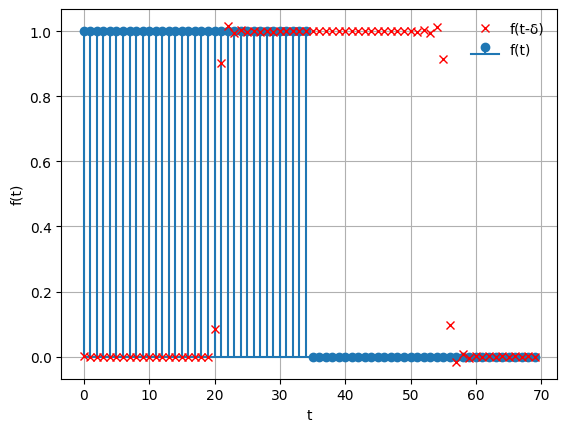
\includegraphics[width=0.4\columnwidth]{images/Results/M_1_small_shift.png}
			\caption{Shift by $20.01$ with $M=1$}
			\label{small_shift_M_1}
		\end{figure}
		
		This result is attributed to the fact that the filter contains fewer oscillations as well. In fact if we take a look at the filter defined for $M=1$ we can see that we have maximum oscillations exactly at $0.5$. 
		This is why for a fractional shift that gets closer to $0.5$ it is necessary to use a bigger value for M such as $\frac{3}{2}$ or $2$ to smooth out the oscillations.
		\begin{figure}[H]
			\centering
			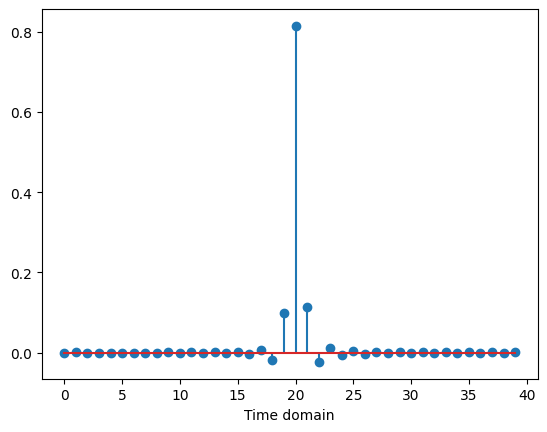
\includegraphics[width=0.3\columnwidth]{images/Results/M_1_filter_small_shift.png}\hspace*{0.2\columnwidth}
			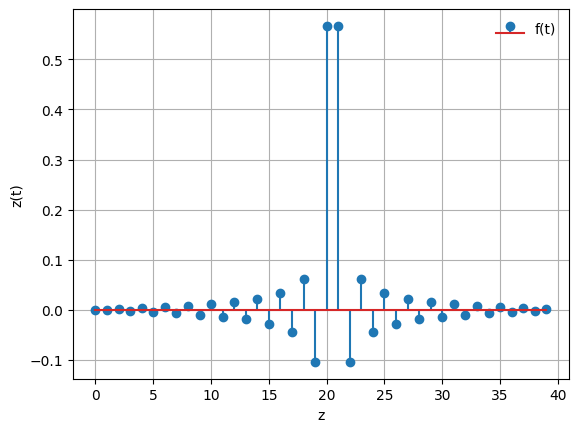
\includegraphics[width=0.3\columnwidth]{images/Results/M_1_filter_big_shift.png}\\
			\parbox{0.3\columnwidth}{\centering Filter shifted by $0.01$ with $M=1$}\hspace*{0.2\columnwidth}
			\parbox{0.3\columnwidth}{\centering Filter shifted by $0.5$ with $M=1$}\\
			\centering
			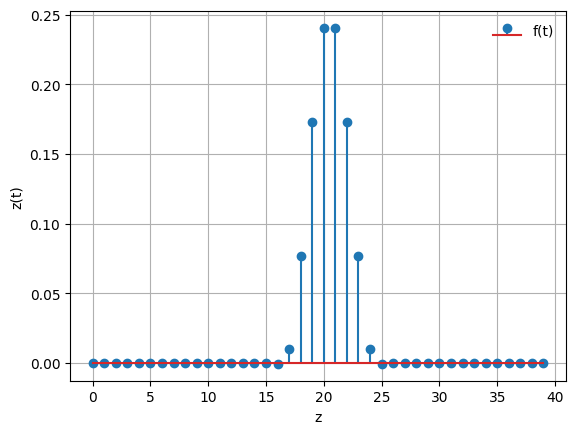
\includegraphics[width=0.3\columnwidth]{images/Results/M_2_filter_big_shift.png}\\
			\parbox{0.3\columnwidth}{\centering Filter shifted by $0.5$ with $M=2$}
			\caption{Difference in oscillations with varying fractional shifts.}
			\label{different_shifts_small_M}
		\end{figure}

		
		\section{Conclusion}
		One way to improve upon this work would be to implement the code with CUDA and a function that chooses which M to use based on the fractional shift and the error.
	
	
	\bibliographystyle{plain}
	\bibliography{references}
	
	
\end{document}